% CeldaUnitaria.m4
\documentclass[ST]{subfiles}
\begin{document}

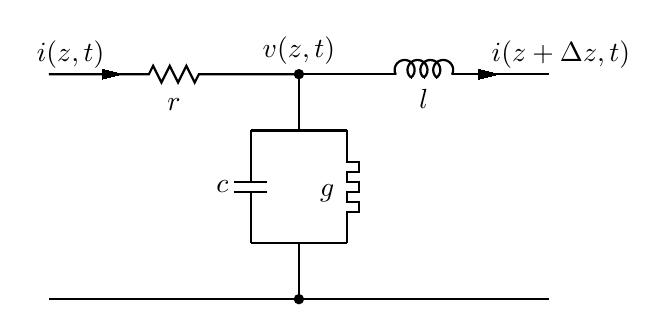
\begin{tikzpicture}[scale=2.54]
% dpic version 2010.11.28 option -g for TikZ and PGF 1.01
\ifx\dpiclw\undefined\newdimen\dpiclw\fi
\global\def\dpicdraw{\draw[line width=\dpiclw]}
\global\def\dpicstop{;}
\dpiclw=0.8bp
\dpiclw=0.8bp
\dpicdraw (0,0)
 --(0.5,0)
 --(0.520833,0.041667)
 --(0.5625,-0.041667)
 --(0.604167,0.041667)
 --(0.645833,-0.041667)
 --(0.6875,0.041667)
 --(0.729167,-0.041667)
 --(0.75,0)
 --(1.25,0)\dpicstop
\draw (0.625,-0.15) node{$ r$};
\filldraw[line width=0bp](0.266667,-0.025)
 --(0.366667,0)
 --(0.266667,0.025) --cycle
\dpicstop
\dpicdraw (0.343761,0)
 --(0.266667,0)\dpicstop
\draw (0.305214,0) node[above left=-1.5bp]{$ i(z,t)$};
\dpicdraw[fill=black](1.25,0) circle (0.007874in)\dpicstop
\draw (1.25,0.02) node[above=-1.5bp]{$ v(z,t)$};
\dpicdraw (1.25,0)
 --(1.25,-0.28125)\dpicstop
\dpicdraw (1.491319,-0.28125)
 --(1.491319,-0.4375)
 --(1.549653,-0.4375)
 --(1.549653,-0.4875)
 --(1.491319,-0.4875)
 --(1.491319,-0.5375)
 --(1.549653,-0.5375)
 --(1.549653,-0.5875)
 --(1.491319,-0.5875)
 --(1.491319,-0.6375)
 --(1.549653,-0.6375)
 --(1.549653,-0.6875)
 --(1.491319,-0.6875)
 --(1.491319,-0.6875)
 --(1.491319,-0.84375)\dpicstop
\draw (1.391319,-0.593333) node{$ g$};
\dpicdraw (1.008681,-0.28125)
 --(1.008681,-0.5375)\dpicstop
\dpicdraw (0.925347,-0.5375)
 --(1.092014,-0.5375)\dpicstop
\dpicdraw (0.925347,-0.5875)
 --(1.092014,-0.5875)\dpicstop
\dpicdraw (1.008681,-0.5875)
 --(1.008681,-0.84375)\dpicstop
\draw (0.925347,-0.5625) node[left=-1.5bp]{$ c$};
\dpicdraw (1.008681,-0.28125)
 --(1.008681,-0.28125)\dpicstop
\dpicdraw (1.008681,-0.28125)
 --(1.491319,-0.28125)\dpicstop
\dpicdraw (1.008681,-0.84375)
 --(1.008681,-0.84375)\dpicstop
\dpicdraw (1.008681,-0.84375)
 --(1.491319,-0.84375)\dpicstop
\dpicdraw (1.25,-0.84375)
 --(1.25,-1.125)\dpicstop
\dpicdraw[fill=black](1.25,-1.125) circle (0.007874in)\dpicstop
\dpicdraw (1.25,0)
 --(1.733266,0)\dpicstop
\dpicdraw[line width=0.4bp](1.733266,-0.002778)
 ..controls (1.735298,-0.002778) and (1.736643,-0.000668)
 ..(1.735784,0.001174)\dpicstop
\dpicdraw (1.733266,-0)
 ..controls (1.715746,0.037572) and (1.748931,0.078918)
 ..(1.789404,0.069946)
 ..controls (1.829877,0.060973) and (1.842478,0.009476)
 ..(1.810721,-0.017171)\dpicstop
\dpicdraw[line width=0.4bp](1.812507,-0.019299)
 ..controls (1.811474,-0.020166) and (1.809968,-0.020166)
 ..(1.808936,-0.019299)\dpicstop
\dpicdraw (1.810721,-0.017171)
 ..controls (1.774962,0.012834) and (1.79618,0.071131)
 ..(1.842861,0.071131)
 ..controls (1.889541,0.071131) and (1.910759,0.012834)
 ..(1.875,-0.017171)\dpicstop
\dpicdraw[line width=0.4bp](1.876786,-0.019299)
 ..controls (1.875753,-0.020166) and (1.874247,-0.020166)
 ..(1.873214,-0.019299)\dpicstop
\dpicdraw (1.875,-0.017171)
 ..controls (1.839241,0.012834) and (1.860459,0.071131)
 ..(1.907139,0.071131)
 ..controls (1.95382,0.071131) and (1.975038,0.012834)
 ..(1.939279,-0.017171)\dpicstop
\dpicdraw[line width=0.4bp](1.941064,-0.019299)
 ..controls (1.940032,-0.020166) and (1.938526,-0.020166)
 ..(1.937493,-0.019299)\dpicstop
\dpicdraw (1.939279,-0.017171)
 ..controls (1.907522,0.009476) and (1.920123,0.060973)
 ..(1.960596,0.069946)
 ..controls (2.001069,0.078918) and (2.034254,0.037572)
 ..(2.016734,-0)\dpicstop
\dpicdraw[line width=0.4bp](2.016734,-0.002778)
 ..controls (2.014702,-0.002778) and (2.013357,-0.000668)
 ..(2.014216,0.001174)\dpicstop
\dpicdraw (2.016734,-0)
 --(2.5,-0)\dpicstop
\draw (1.875,-0.12302) node{$ l$};
\filldraw[line width=0bp](2.147612,-0.025)
 --(2.247612,0)
 --(2.147612,0.025) --cycle
\dpicstop
\dpicdraw (2.224706,0)
 --(2.147612,0)\dpicstop
\draw (2.186159,0) node[above right=-1.5bp]{$ i(z+\Delta z,t)$};
\dpicdraw (2.5,-1.125)
 --(0,-1.125)\dpicstop
\end{tikzpicture}
\end{document}


